\documentclass[UTF8,zihao=-4]{ctexart}
\usepackage[a4paper,margin=2.5cm]{geometry}
\usepackage{amsmath, amssymb, amsthm}
\usepackage{bm}
\usepackage{hyperref}
\usepackage{graphicx}
\usepackage{caption}
\usepackage{listings}
\usepackage{xcolor}
\usepackage{float}
\usepackage{placeins}
\graphicspath{{figures/}}

% Code style
\lstdefinestyle{code}{
  basicstyle=\ttfamily\small,
  numbers=left,
  numberstyle=\tiny,
  numbersep=8pt,
  keywordstyle=\color{blue},
  commentstyle=\color{teal!70!black},
  stringstyle=\color{orange!70!black},
  showstringspaces=false,
  breaklines=true,
  frame=single,
  framerule=0.3pt,
  rulecolor=\color{black!15}
}
\lstset{style=code}

\title{模型训练与参数调优策略}
\author{}
\date{\today}

\begin{document}
\maketitle
\tableofcontents
\FloatBarrier

\section{超参数选择:批大小、学习率与优化器}
超参数决定了优化的几何性质与模型的泛化表现。良好的默认配置可以显著减少调参压力,而可解释的缩放规律则帮助我们在硬件预算变化时快速迁移经验。图~\ref{fig:hyperparameter_landscape_cn} 展示了学习率、批大小与优化器之间的典型相互作用。

\subsection{批大小}
批大小 $B$ 在统计效率与硬件吞吐之间折衷。梯度噪声尺度 $\mathcal{G}$ 描述了随机性随批大小的变化:
\begin{equation}
  \mathcal{G} = \frac{\mathbb{E}\bigl[\|\nabla \mathcal{L}(\boldsymbol{\theta}; \mathcal{B})\|_2^2\bigr] - \|\nabla \mathcal{L}(\boldsymbol{\theta})\|_2^2}{\|\nabla \mathcal{L}(\boldsymbol{\theta})\|_2^2}.
\end{equation}
当 $B \gg \mathcal{G}$ 时,梯度方差的下降趋于饱和,继续增大批量只会提高显存占用而难以提升收敛速度。在显存受限时可通过梯度累积模拟大批量训练,并结合梯度裁剪防止累积过程中出现梯度爆炸。

\subsection{学习率策略}
``线性缩放法则'' 建议在将批大小从 $B_0$ 增大到 $B$ 时,学习率按 $\eta \approx \eta_0 \cdot B / B_0$ 缩放。但为了稳定性,必须配合 warm-up:
\begin{equation}
  \eta_t =
  \begin{cases}
    \eta_{\text{target}} \frac{t}{T_w}, & 0 \le t \le T_w, \\
    \eta_{\text{schedule}}(t - T_w), & t > T_w.
  \end{cases}
\end{equation}
余弦退火、逆平方衰减、循环学习率等自适应策略能够在训练前期快速下降、后期平稳收敛。学习率区间测试(LR range test)通过指数扫描学习率,快速定位可训练范围。

\subsection{优化器选择}
不同优化器对应了梯度到参数更新的不同映射方式:
\begin{itemize}
  \item \textbf{带动量的 SGD:} 适合大规模视觉任务,通过 $\mathbf{v}_{t+1} = \mu \mathbf{v}_t + \nabla_{\boldsymbol{\theta}} \mathcal{L}_t$ 与 $\boldsymbol{\theta}_{t+1} = \boldsymbol{\theta}_t - \eta \mathbf{v}_{t+1}$ 抑制狭长峡谷中的振荡。
  \item \textbf{AdamW:} 维护每个参数的一阶、二阶矩并解耦权重衰减,是语言模型与稀疏梯度任务的主流选择。
  \item \textbf{Lion、LAMB、Adafactor:} 面向超大 transformer 的硬件友好优化器,引入层级缩放、低内存矩估计等改进。
\end{itemize}
混合精度训练会影响动量统计的估计,因此通常在优化器 step 之前执行梯度裁剪,并确保动态 loss scaling 的溢出处理不会破坏梯度分布。

\subsection{搜索策略}
随机搜索与贝叶斯优化是强力基线。定义搜索空间 $\mathcal{S}$ 时,对学习率等尺度敏感参数采用对数均匀分布(如 $\log_{10} \eta \sim U[-5, -1]$)。连续减半(Successive Halving)与种群式训练(Population-Based Training)可在有限算力下快速淘汰低效配置。下面给出一个简单的随机搜索示例:

\begin{lstlisting}[language=Python, caption={批大小、学习率与优化器的随机搜索示例。}]
import random
from itertools import count

search_space = {
    "batch_size": [64, 128, 256, 512],
    "lr": lambda: 10 ** random.uniform(-4.5, -2.5),
    "optimizer": lambda: random.choice(["sgd_momentum", "adamw", "lion"]),
}

def sample_config():
    return {
        "batch_size": random.choice(search_space["batch_size"]),
        "lr": search_space["lr"](),
        "optimizer": search_space["optimizer"](),
    }

best = None
for trial in count(start=1):
    cfg = sample_config()
    metrics = train_and_evaluate(cfg)  # 用户实现
    if best is None or metrics["val_accuracy"] > best["val_accuracy"]:
        best = {"trial": trial, **cfg, **metrics}
    if stopping_criterion(best, trial):
        break

print(f"Best config: {best}")
\end{lstlisting}

\begin{figure}[H]
  \centering
  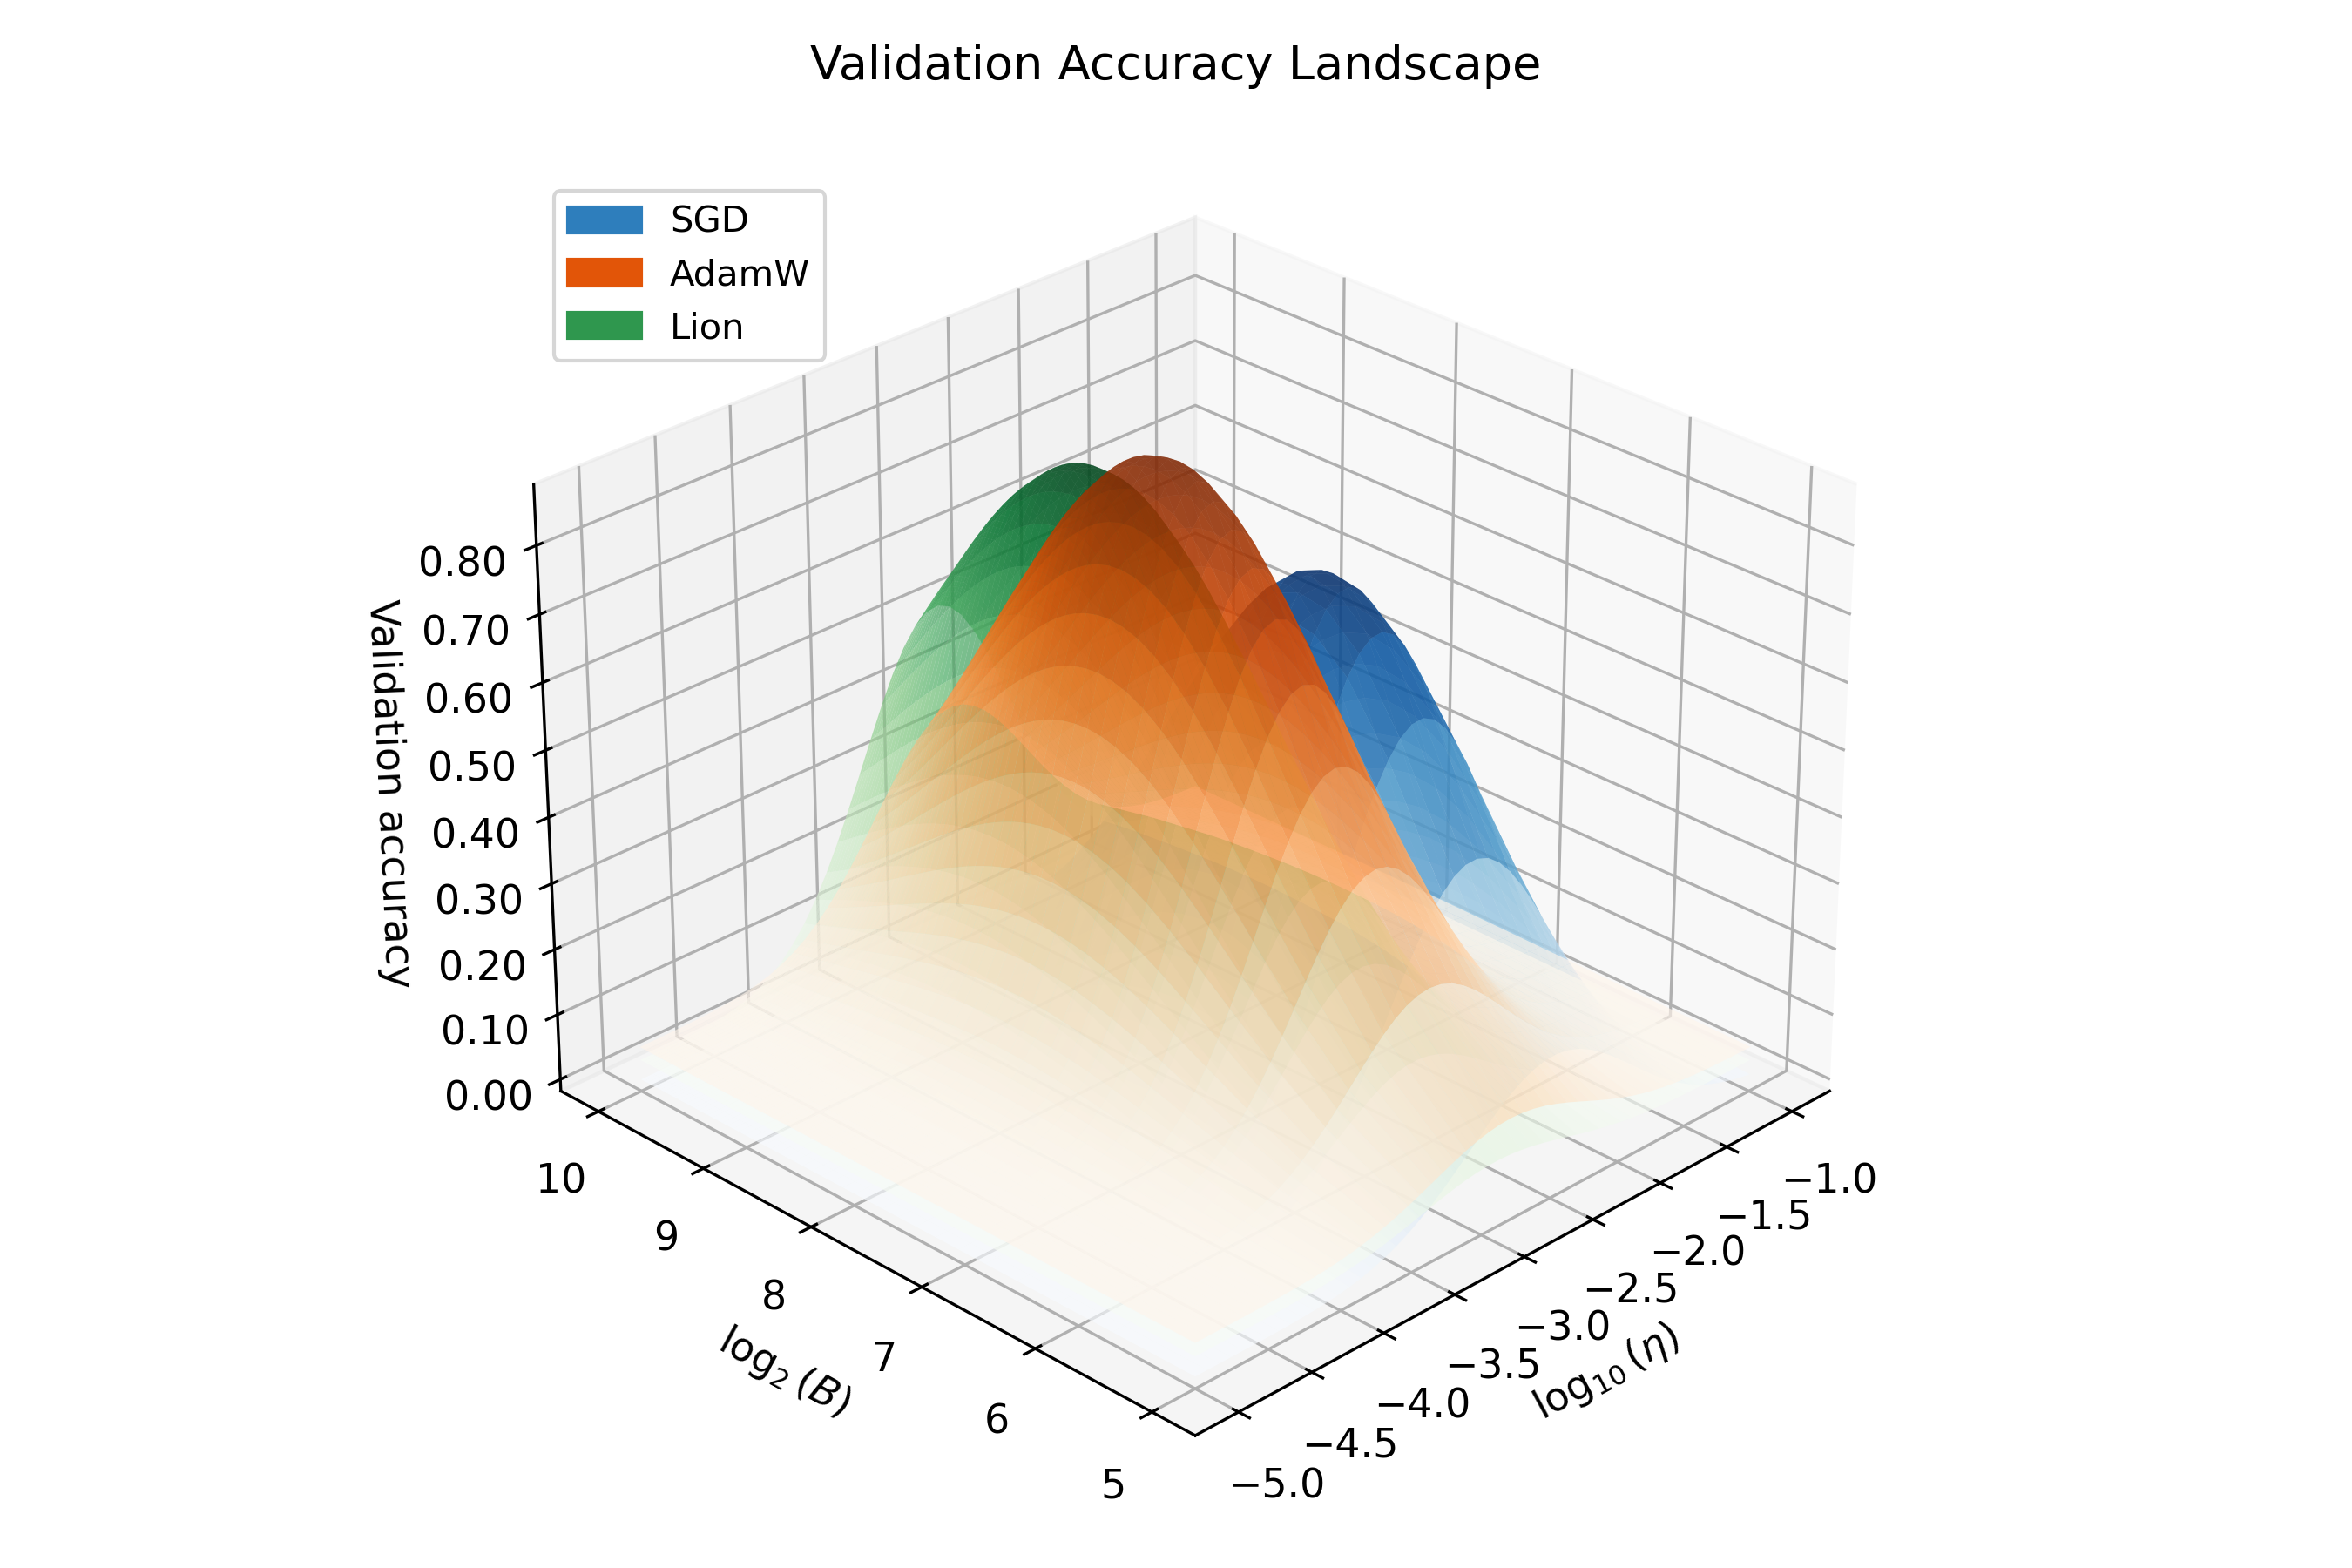
\includegraphics[width=0.85\textwidth]{hyperparameter_landscape.png}
  \caption{不同学习率、批大小与优化器组合的验证性能。前沿面展示了兼顾速度与泛化的配置区域。}
  \label{fig:hyperparameter_landscape_cn}
\end{figure}
\FloatBarrier

\section{Early Stopping 与 Checkpoint 策略}
Early stopping 通过监控验证指标及时停止训练,避免过拟合;Checkpoint 机制则用于恢复、集成或继续微调。图~\ref{fig:early_stopping_checkpoint_cn} 概括了常见流程。

\subsection{基于耐心值的 Early Stopping}
设验证指标为 $m_t$,耐心值为 $p$,最小提升阈值为 $\delta$,若
\begin{equation}
  \max_{t - p \le k \le t} m_k \le m_{t-p} + \delta
\end{equation}
持续 $p$ 个评估周期,则在步骤 $t^\star$ 触发停止。恢复到最佳 checkpoint 可以保留训练中期获得的最佳泛化性能。使用指数滑动平均平滑验证曲线,可减少噪声引发的误触发。

\subsection{Checkpoint 策略}
Checkpoint 的保存频率需要在存储与鲁棒性之间权衡:
\begin{itemize}
  \item \textbf{滑动窗口:} 只保留最近 $K$ 个 checkpoint,及时清理旧文件。
  \item \textbf{最佳集合:} 保存性能最优的若干模型,便于后续集成或蒸馏。
  \item \textbf{事件触发:} 指标提升超过阈值、epoch 翻倍或阶段性里程碑时触发保存。
\end{itemize}
要完整恢复训练状态,需要保存优化器状态(动量、二阶矩)以及学习率调度器的内部计数。针对超大模型,可使用分片格式(如 FSDP Shard、TensorFlow Checkpoint Shard)降低单节点内存压力。

\subsection{与超参搜索的结合}
在异步超参搜索中,早停可以加速淘汰效果不佳的试验。Population-Based Training 会周期性地用表现最佳的配置去替换低效个体,因此需要轻量化的 checkpoint 以降低复制延迟。

\subsection{示例实现}

\begin{lstlisting}[language=Python, caption={PyTorch 环境下的 Early Stopping 与 Checkpoint 轮换。}]
import torch
from pathlib import Path

def save_checkpoint(path: Path, model, optimizer, step: int, metrics: dict):
    state = {
        "model": model.state_dict(),
        "optimizer": optimizer.state_dict(),
        "step": step,
        "metrics": metrics,
    }
    torch.save(state, path)

def early_stopping_loop(dataloader, model, optimizer, scheduler, patience=10, min_delta=1e-4):
    best_metric = -float("inf")
    best_path = Path("checkpoints/best.pt")
    wait = 0
    for step, batch in enumerate(dataloader, start=1):
        train_step(model, optimizer, batch)
        if step % 100 == 0:
            metric = evaluate_validation(model)
            scheduler.step(metric)
            save_checkpoint(Path(f"checkpoints/step_{step}.pt"), model, optimizer, step, {"val": metric})
            rotate_checkpoints(Path("checkpoints"), keep=3)
            if metric > best_metric + min_delta:
                best_metric = metric
                wait = 0
                save_checkpoint(best_path, model, optimizer, step, {"val": metric})
            else:
                wait += 1
                if wait >= patience:
                    restore_checkpoint(best_path, model, optimizer)
                    print(f"Early stop at step {step}, best metric {best_metric:.4f}")
                    break
\end{lstlisting}

\begin{figure}[H]
  \centering
  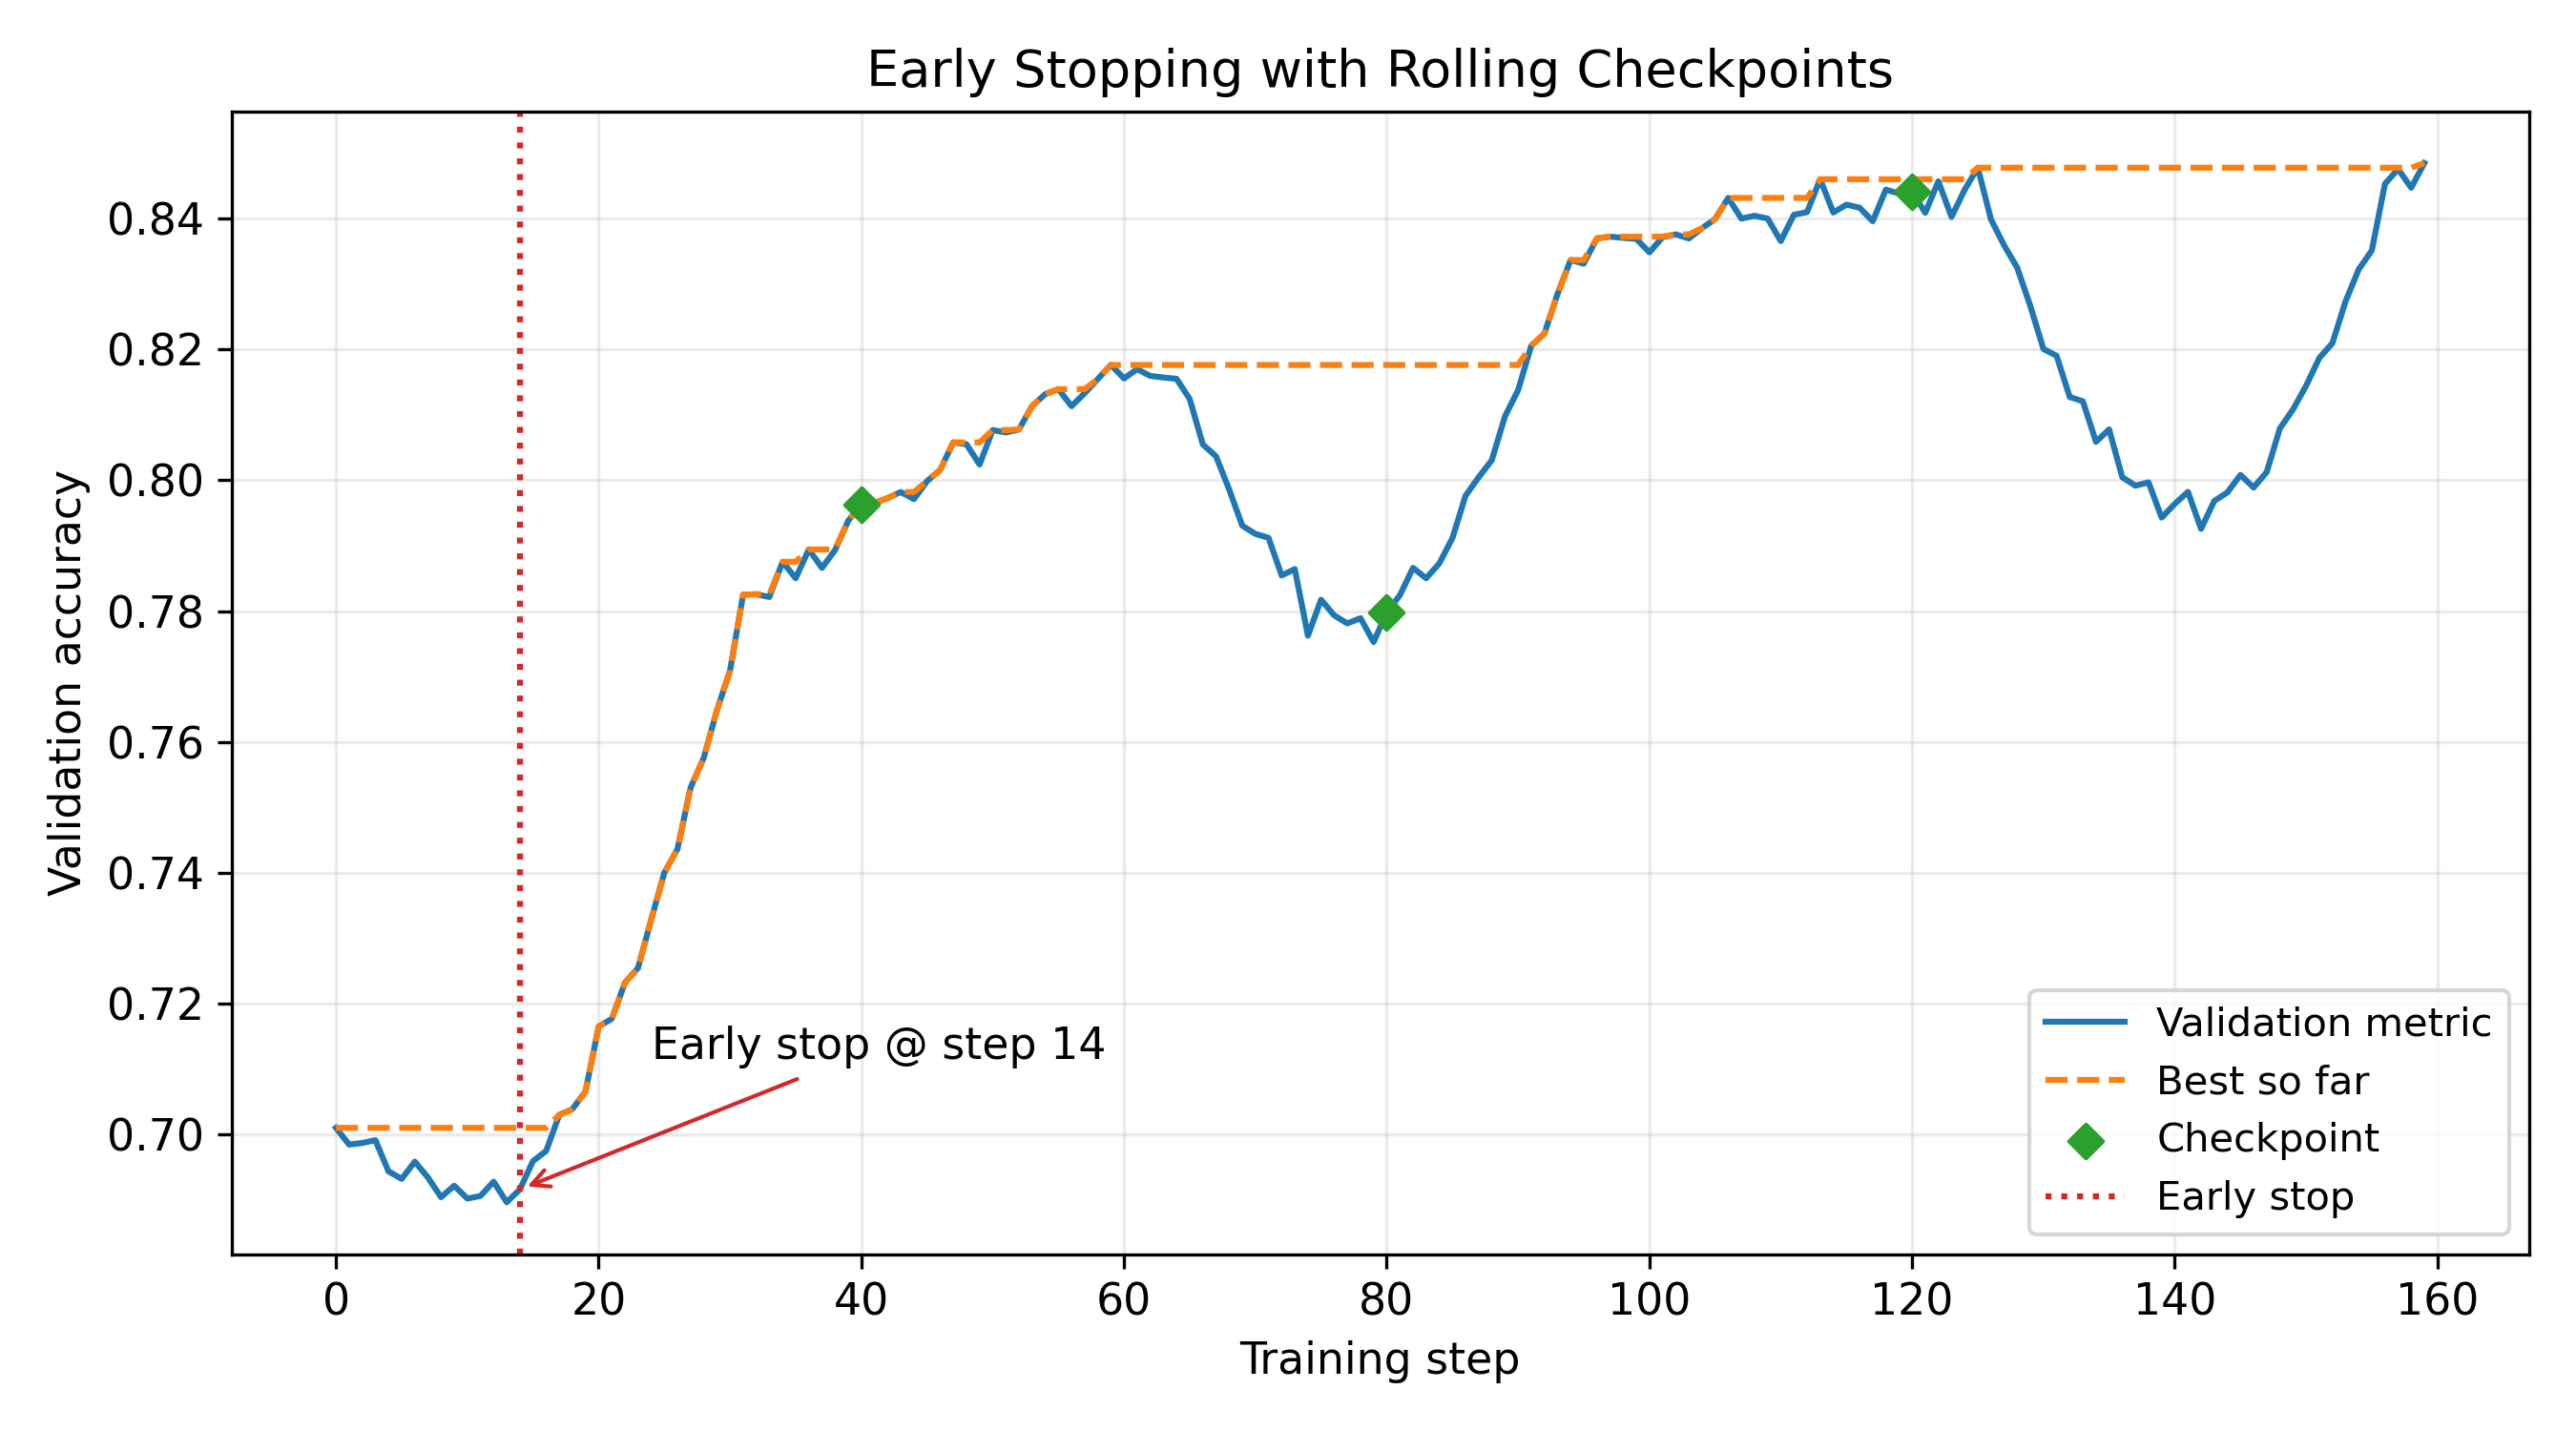
\includegraphics[width=0.85\textwidth]{early_stopping_checkpoint.png}
  \caption{带有 Early Stopping 的验证指标演化轨迹。最佳 checkpoint 在过拟合出现前被捕获,并可用于集成或热重启。}
  \label{fig:early_stopping_checkpoint_cn}
\end{figure}
\FloatBarrier

\section{大规模训练与分布式并行}
超大模型的训练需要跨多 GPU/TPU、乃至多节点集群协同完成。合理的并行策略必须在计算、通信和内存之间取得平衡。图~\ref{fig:distributed_training_topologies_cn} 对比了常见拓扑结构,图~\ref{fig:scaling_efficiency_cn} 展示了弱、强缩放效率。

\subsection{数据并行}
数据并行在 $N$ 个工作节点上复制完整模型,各自处理不同 mini-batch,并通过 all-reduce 聚合梯度:
\begin{equation}
  \boldsymbol{\theta}_{t+1} = \boldsymbol{\theta}_t - \eta \frac{1}{N} \sum_{n=1}^{N} \nabla_{\boldsymbol{\theta}} \mathcal{L}_t^{(n)}.
\end{equation}
通信复杂度随参数量 $P$ 与 $\log N$ 增长。梯度压缩、混合精度通信、通信-计算重叠等技巧能够缓解带宽瓶颈。

\subsection{模型并行与流水线并行}
当模型无法放入单个设备时,可以按张量或层级进行拆分:
\begin{itemize}
  \item \textbf{张量并行:} 将矩阵乘法沿特定维度划分,多卡协同完成(如 Megatron-LM)。
  \item \textbf{流水线并行:} 将网络切成若干 stage,使用微批次(micro-batch)流水传递,典型调度包括 1F1B、交错流水等。
\end{itemize}
混合并行结合数据、模型与流水线并行,支撑万亿参数级模型。需要注意负载均衡、防止流水空泡以及调度器同步开销。

\subsection{同步与容错}
大规模集群中拖慢节点(straggler)与故障不可避免。弹性训练框架(Horovod Elastic、TorchElastic)允许节点动态加入/退出。参数服务器式的异步更新提高吞吐,但会引入陈旧梯度,可通过延迟上界与自适应学习率缓解。

\subsection{性能建模}
加速比 $S(N)$ 与并行效率 $E(N) = S(N) / N$ 是常用指标:
\begin{equation}
  S(N) = \frac{T(1)}{T(N)}, \qquad E(N) = \frac{T(1)}{N \cdot T(N)}.
\end{equation}
Roofline 模型从算力与带宽上界刻画可达性能。分析工具(Nsight Systems、PyTorch Profiler)可定位内核级热点与通信瓶颈。

\subsection{分布式训练骨架}

\begin{lstlisting}[language=Python, caption={PyTorch 分布式数据并行骨架,带弹性重启钩子。}]
import os
import torch
import torch.distributed as dist
from torch.nn.parallel import DistributedDataParallel as DDP

def setup_distributed():
    dist.init_process_group(backend="nccl")
    torch.cuda.set_device(int(os.environ["LOCAL_RANK"]))

def train(rank):
    setup_distributed()
    model = build_model().cuda()
    ddp_model = DDP(model, device_ids=[int(os.environ["LOCAL_RANK"])])
    optimizer = torch.optim.AdamW(ddp_model.parameters(), lr=2e-4)
    scaler = torch.cuda.amp.GradScaler()

    train_loader = build_dataloader(distributed=True)
    for epoch in range(num_epochs()):
        train_loader.sampler.set_epoch(epoch)
        for batch in train_loader:
            optimizer.zero_grad(set_to_none=True)
            with torch.cuda.amp.autocast():
                loss = ddp_model(batch["inputs"]).loss
            scaler.scale(loss).backward()
            scaler.unscale_(optimizer)
            torch.nn.utils.clip_grad_norm_(ddp_model.parameters(), max_norm=1.0)
            scaler.step(optimizer)
            scaler.update()
        if dist.get_rank() == 0:
            save_checkpoint_sharded(ddp_model, optimizer, epoch)

    dist.destroy_process_group()
\end{lstlisting}

\begin{figure}[H]
  \centering
  
\includegraphics[width=0.9\textwidth]{distributed_training_topologies.png}
  \caption{数据并行、流水线并行与混合并行的拓扑对比。箭头表示激活与梯度的传递方向以及同步位置。}
  \label{fig:distributed_training_topologies_cn}
\end{figure}

\begin{figure}[H]
  \centering
  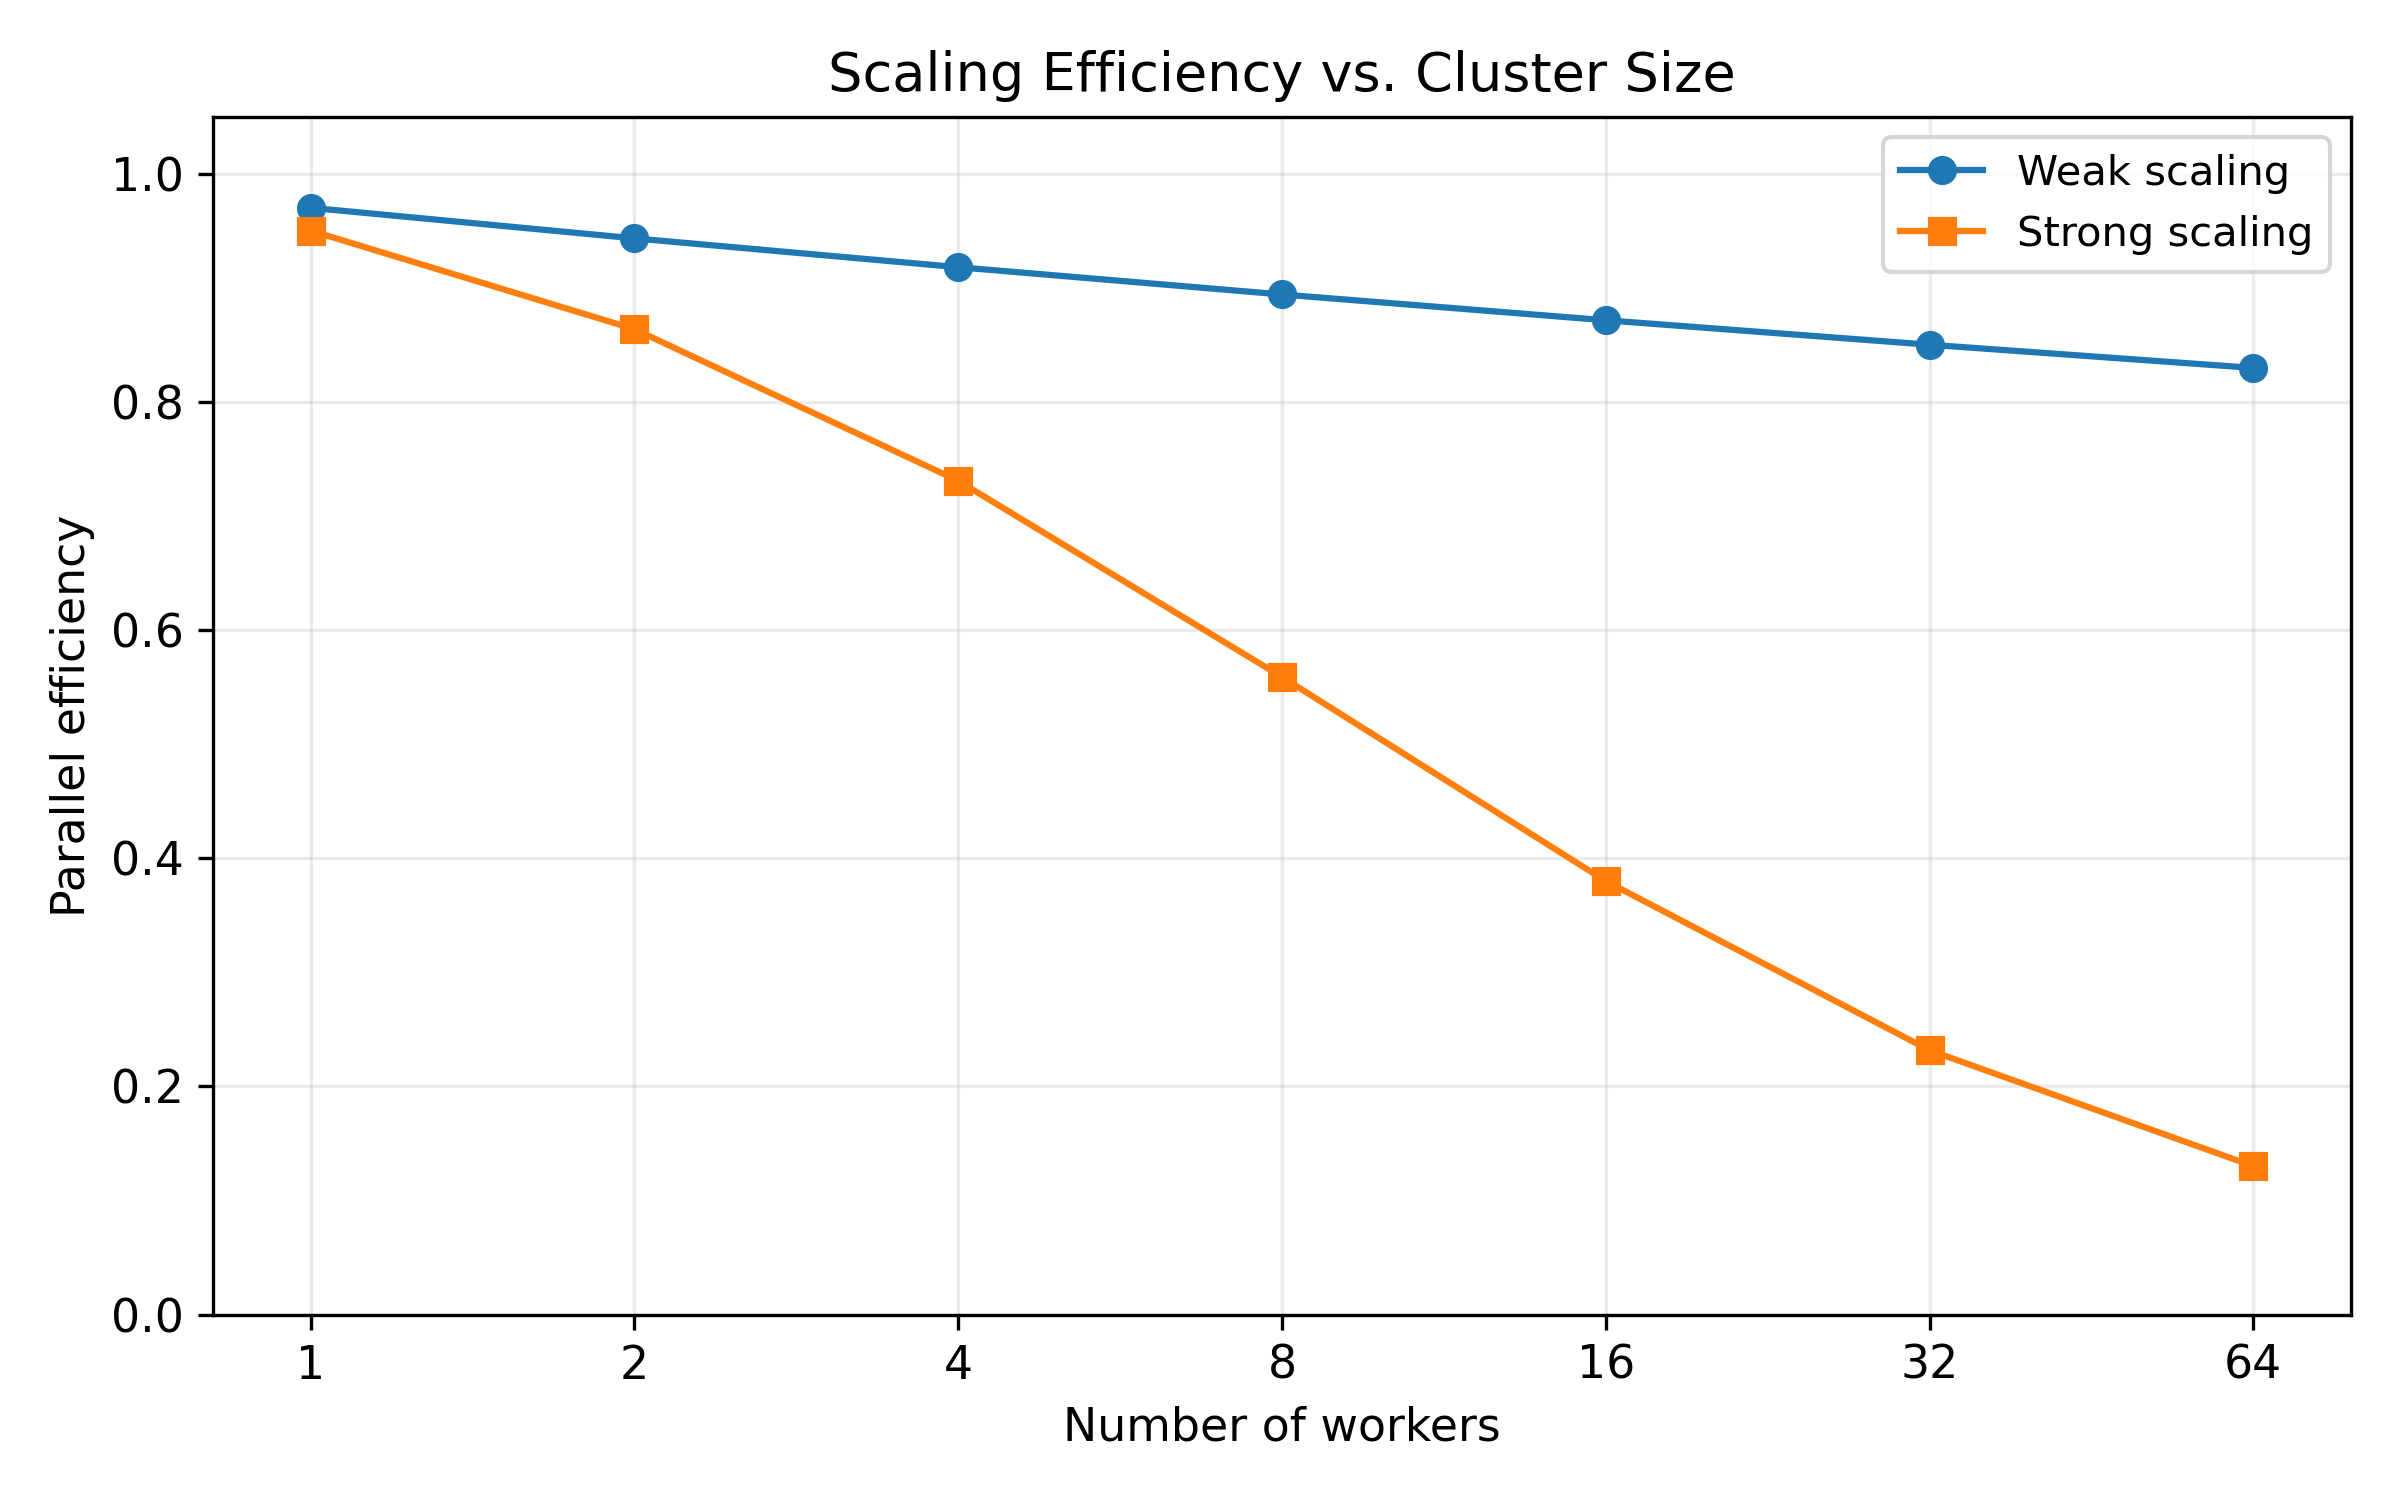
\includegraphics[width=0.85\textwidth]{scaling_efficiency.png}
  \caption{弱缩放与强缩放实验的效率曲线。通信优化后的配置在大规模节点上保持更高效率。}
  \label{fig:scaling_efficiency_cn}
\end{figure}
\FloatBarrier

\section*{延伸阅读}
\begin{itemize}
  \item Priya Goyal 等:《Accurate, Large Minibatch SGD: Training ImageNet in 1 Hour》,2017。
  \item Nitish S. Keskar 等:《On Large-Batch Training for Deep Learning》,ICLR 2017。
  \item Chen Ying 等:《A Survey on Distributed Training of Deep Learning Models》,2022。
  \item Rich Caruana 等:《Ensemble Selection from Libraries of Models》,ICML 2004。
\end{itemize}

\end{document}
